First, we need to define a similarity function that measures "how much our points are similar to each other". Let \(X_i\) and \(X_j\) be two points in our data, then we will use a similarity measure defined as:
\begin{equation}
  s_{i,j} = \exp \left(- \frac{\| X_i- X_j \|^2}{2\sigma^2}\right)
\end{equation}
Then, a \textit{\(K\)-Nearest Neighborhood} similarity graph is a Graph \(G= (V,E)\) where each vertex \(v_1, \dots v_n\) represents a point and two vertices \(v_i\) and \(v_j\) are connected by an undirected edge \(e_{i,j}\) if the similarity between \(v_i\) and \(v_j\) is among the \(K\)-th highest similarities between \(v_i\) and other vertices in \(V\). For such graph we can define the relative adjacency matrix as \(W_{i,j} = s_{i,j}\) where each entry \(W_{i,j}\) is nonzero only if there exists an edge between \(v_i\) and \(v_j\). \(W\) has zero-values on the diagonal by definition.
\\
\\
The following MATLAB code was use to generate the K-NN similarity graph of our data:
\lstinputlisting{../knn_graph.m}
Running \texttt{knn\_graph} on both dataset using \(\sigma= 1\) and testing with \(K= 10, 20, 40\) gave the following results:
\begin{figure}[H]
  \centering
  \subfloat[1][\(K= 10\)]{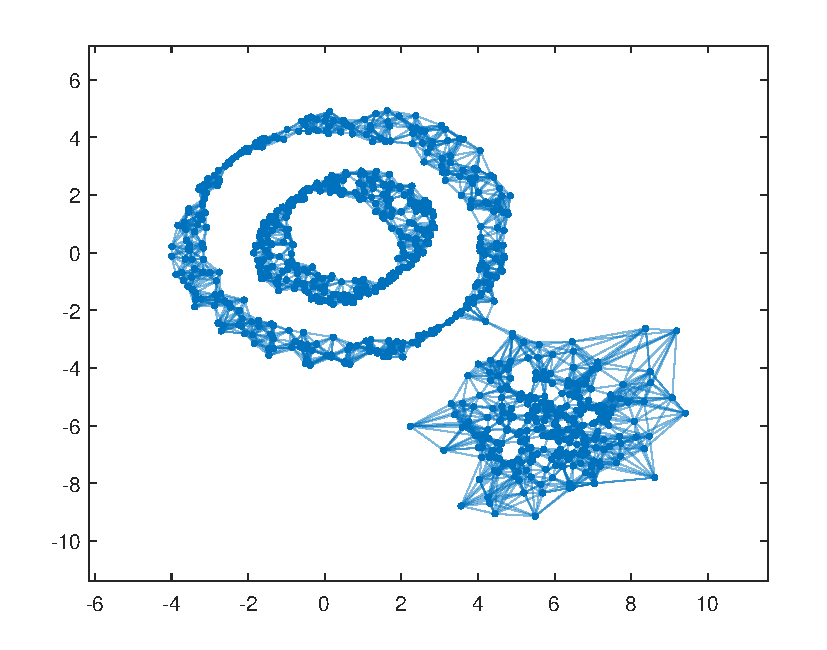
\includegraphics[scale = 0.37]{pictures/circle_KNN_K10.pdf}}
  \subfloat[2][\(K= 20\)]{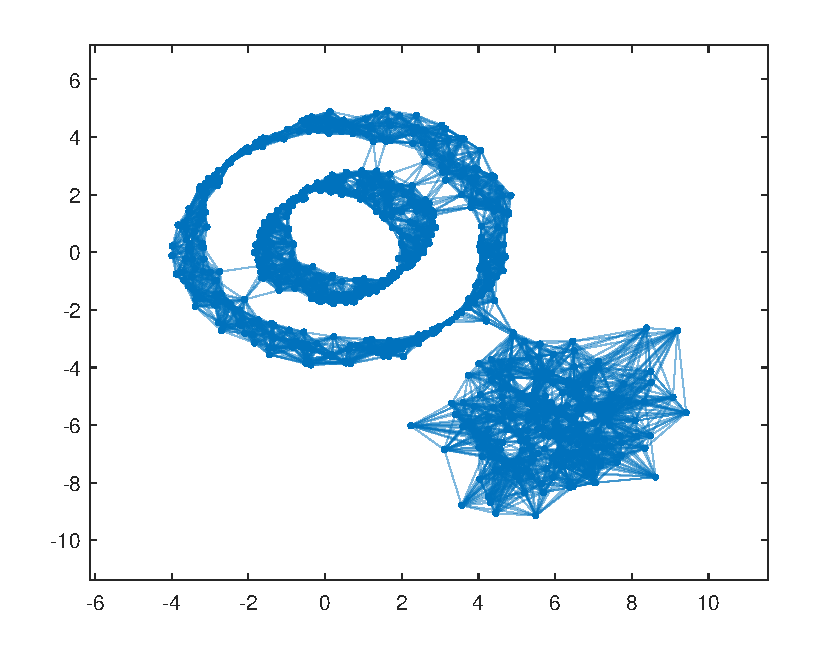
\includegraphics[scale = 0.37]{pictures/circle_KNN_K20.pdf}}
  \subfloat[3][\(K= 40\)]{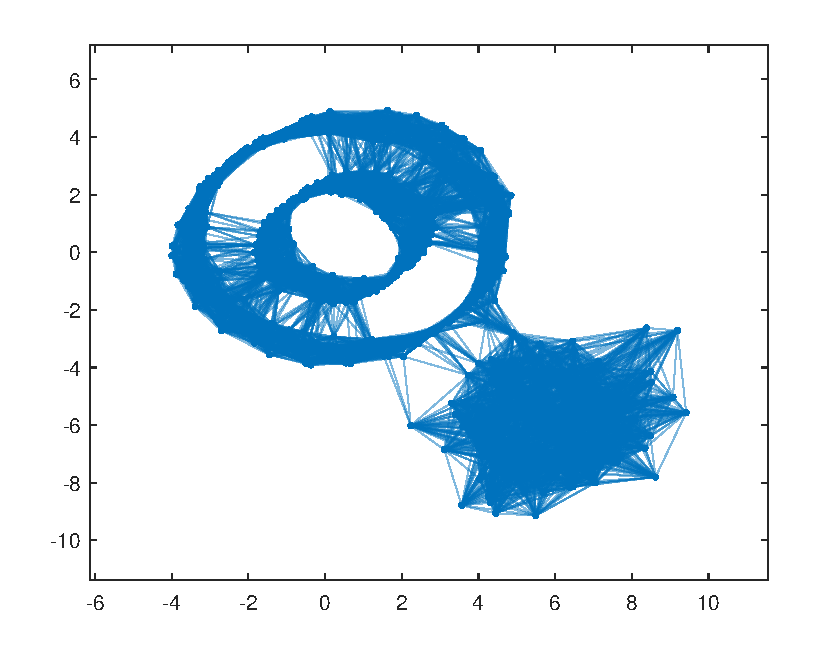
\includegraphics[scale = 0.37]{pictures/circle_KNN_K40.pdf}}
  \caption{K-NN graphs plots for \texttt{Circle} data with different values of \(K\)}
  \label{KNN_circle}
\end{figure}
\begin{figure}[H]
  \centering
  \subfloat[1][\(K= 10\)]{\includegraphics[scale = 0.37]{pictures/spiral_KNN_K10.pdf}}
  \subfloat[2][\(K= 20\)]{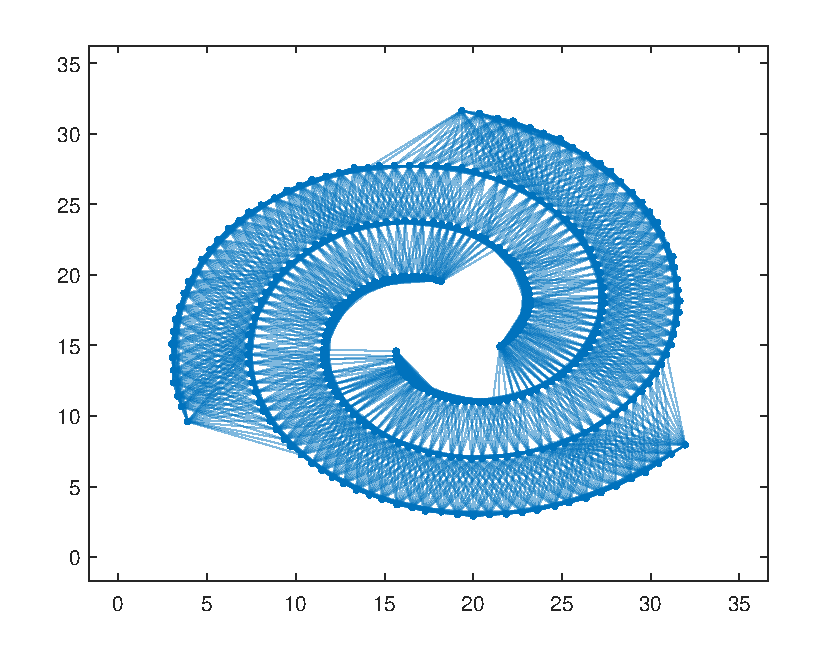
\includegraphics[scale = 0.37]{pictures/spiral_KNN_K20.pdf}}
  \subfloat[3][\(K= 40\)]{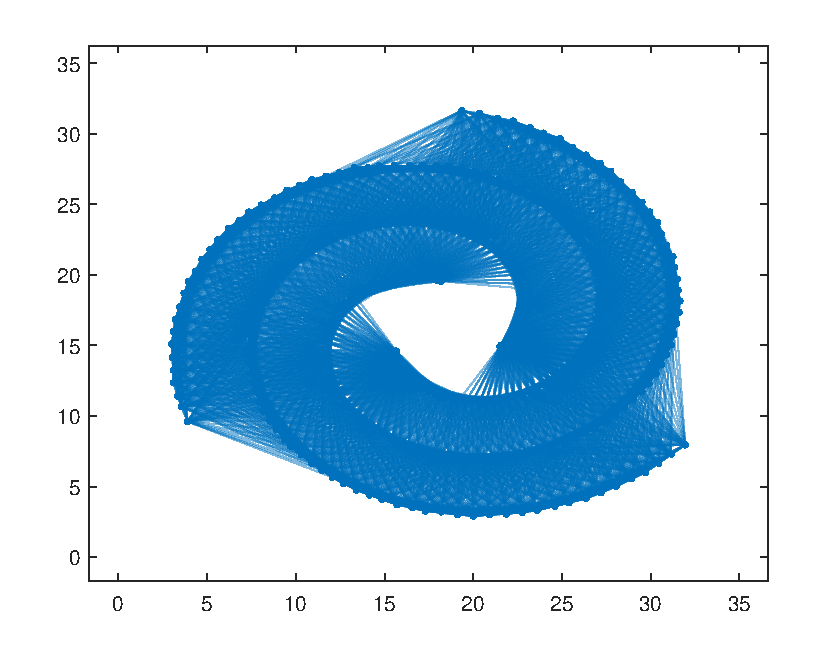
\includegraphics[scale = 0.37]{pictures/spiral_KNN_K40.pdf}}
  \caption{K-NN graphs plots for \texttt{Spiral} data with different values of \(K\)}
  \label{KNN_spiral}
\end{figure}

Our objective is to find a K-NN graph that "separates well" the shapes, meaning that in the best case each shape is a connected component of the graph. As we can see, for both \texttt{Circle} and \texttt{Spiral} data, the value \(K = 10\) seems to separate the shapes well. We will quantify the concept of \textit{good cluster separation} in the next section.